\documentclass{ieeeojies}
\usepackage{cite}
\usepackage{amsmath,amssymb,amsfonts}
\usepackage{algorithmic}
\usepackage{graphicx}
\usepackage{textcomp}
\usepackage{array}
\usepackage[table]{xcolor}
\usepackage{multirow}
\usepackage{multicol}
\usepackage{float}
\usepackage{hyperref}
\usepackage{indentfirst}
% package 2 pic in one row
\usepackage{subfigure}

\setlength{\parindent}{0.5cm}
\def\BibTeX{{\rm B\kern-.05em{\sc i\kern-.025em b}\kern-.08em
    T\kern-.1667em\lower.7ex\hbox{E}\kern-.125emX}}


\begin{document}
\title{PREDICTIVE MODELING OF VIETNAMESE BANK STOCKS: ASSESSING STATISTICAL, MACHINE LEARNING, AND DEEP LEARNING TECHNIQUES}

\author{\uppercase{Tran Truc Quynh}\authorrefmark{1},
\uppercase{Luong Thi Thuy Diem\authorrefmark{2}, and Nguyen Huu Thanh}\authorrefmark{3}}

\address[1]{Faculty of Information Systems, University of Information Technology, (e-mail: 21522539@gm.uit.edu.vn)}
\address[2]{Faculty of Information Systems, University of Information Technology, (e-mail: 21521953@gm.uit.edu.vn)}
\address[3]{Faculty of Information Systems, University of Information Technology, (e-mail: 21522599@gm.uit.edu.vn)}

\markboth
{Author \headeretal: Tran Truc Quynh,Nguyen Huu Thanh,Luong Thi Thuy Diem}
{Author \headeretal: Tran Truc Quynh,Nguyen Huu Thanh,Luong Thi Thuy Diem}

\begin{abstract}
The volatility of stock prices presents challenges for investors navigating the Vietnamese market, which has witnessed increased participation in recent years. This paper seeks to empower investors by evaluating the effectiveness of different forecasting models—specifically Linear Regression, ARIMA, RNN, GRU, LSTM, FFT, XGBoost, and FCN — in predicting price trends for three prominent bank stocks (ACB, BIDV, VCB) traded on the Hochiminh Stock Exchange (HOSE) over a five-year period (2019-2024). Through rigorous analysis and comparison using metrics such as RMSE, MAPE, and MAE. This study identifies the most effective forecasting model for each bank stock. Additionally, it evaluates the impact of different training/test ratio configurations on model performance, providing insights into optimal data partitioning strategies. The main contribution of this study is to provide investors with a comparative analysis of forecasting models, thereby equipping them with insights for informed stock selection and enhancing decision-making accuracy.

\end{abstract}

\begin{keywords}
Model Performance Evaluation, Optimal Forecasting Model Selection, Financial Forecasting, Vietnamese Stock Market, GRU, RNN, ARIMA, LSTM, FFT, XGBoost, FCN, Linear Regression.
\end{keywords}

\titlepgskip=-15pt

\maketitle
\section{Introduction}% \label{sec:introduction}
The Vietnamese stock market has experienced significant growth and increased investor participation in recent years, highlighting its potential and the overall economic recovery post-2023. However, the inherent volatility of stock prices presents challenges for investors, particularly in the banking sector, which is a crucial pillar of the economy. This study aims to assist investors by evaluating the effectiveness of various forecasting models in predicting stock price trends for three major banks—Asia Commercial Bank (ACB), Bank for Investment and Development of Vietnam (BIDV), and Joint Stock Commercial Bank for Foreign Trade of Vietnam (VCB)—listed on the Hochiminh Stock Exchange (HOSE).

To achieve this, we applied a range of statistical, machine learning, and deep learning models, including Linear Regression, ARIMA, RNN, GRU, LSTM, FFT, XGBoost, and FCN, to historical stock price data from 2019 to 2024. Our methodology involved a comprehensive assessment using metrics like RMSE, MAPE, and MAE to determine the accuracy and reliability of each model. Additionally, we explored the effects of varying training/test ratio configurations on the performance of these models, offering valuable insights into effective data partitioning strategies.

The core contribution of this research lies in its detailed comparison of these forecasting models, providing investors with crucial information for making informed stock selection decisions. By pinpointing the most effective model for each bank stock, we aim to support investors in navigating the complex and fluctuating Vietnamese stock market with greater confidence and precision.
\section{Related Works}
Over the past several years, a significant volume of research has concentrated on forecasting stock prices by leveraging various machine learning and statistical techniques.

Maqsood et al. have used linear regression and 2 models for stock exchange forecasting \cite{cakra2015stock}. Meanwhile, URAS combined linear regression and neural network models to forecast Bitcoin closing prices, showing that linear regression had faster execution speed and could accurately predict Bitcoin price fluctuations \cite{uras2020forecasting}.

Manish Dadhich studied and applied the ARIMA model for short-term forecasting of BSE and NSE stock prices. After carrying out his research, Manish Dadhich demonstrated the strength of the ARIMA model in predicting daily closing prices of time series data \cite{dadhich2021predictive}. In Anusha Garlapati's research, she also used ARIMA to forecast stock prices and concluded that ARIMA is a good model for predicting stock prices \cite{garlapati2021stock}.

Yongqiong Zhu \cite{ZhuRNN} applied an RNN model to predict the stock prices of Apple. The training dataset spanned 10 years with 65\% allocated for training and the remaining 3\% for testing. With 50 epochs, Adam optimization, and Mean Squared Error (MSE) as the loss function, the model achieved highly favorable outcomes. It attained a predictive accuracy exceeding 95\%, with a reported loss value of 0.1\%. In 2015, Xiao Ding \cite{DingGRU} also proposed a deep learning method for event-driven stock market prediction.

Shejul et al. \cite{ShejulGRU} compared the performance of the Gated Recurrent Unit (GRU) and Bidirectional Long Short-Term Memory (BiLSTM) models in predicting stock prices. Experimental results indicate that both models accurately forecast future stock prices, with the BiLSTM model outperforming the GRU model. Despite this, the GRU model demonstrates nearly double the speed of the BiLSTM model due to its simpler architecture. Overall, both models offer precise predictions and can effectively anticipate future stock market trends.

C. Fjellström (2022) \cite{fjellstrom2022lstm} demonstrates the effectiveness of LSTMs in capturing the complexities of financial time series data in the paper "Long Short-Term Memory Neural Network for Financial Time Series." With details the data preprocessing steps, network architecture, and training/testing processes comprehensively, making it replicable for future researchers. However the paper lack of comparison with other advanced machine learning models

Chen et al.\cite{ChenFFT} used an Fast Fourier Transform algorithm to deal with historical training data for forecasting stock prices, achieving a more highly accurate. Experimental analysis is performed on datasets covering a seven-year period of both the Taiwan Stock Exchange Capitalization Weighted Stock Index (TAIEX) and the Dow-Jones Industrial Average (DJIA). 

Tianqi Chen and Carlos Guestrin (2016)\cite{chen2016xgboost} introduced XGBoost, a scalable tree boosting system. The primary contribution of this paper is the development of a highly scalable and efficient tree boosting system. XGBoost can handle billions of examples and is optimized for both single-machine and distributed computing environments

Fully Convolutional Networks (FCNs) have been studied and applied in various fields related to image data processing and semantic segmentation. According to Shima Nabiee's research on stock trend prediction, FCNs have also been proven to be a powerful and flexible tool, enabling the analysis and prediction of stock price trends based on raw data \cite{nabiee2023stock}.
\section{Materials}
\subsection{Dataset}

The analysis will focus on the historical stock prices of three banks in Vietnam: the Asia Commercial Joint Stock Bank (ACB), the Bank for Investment and Development of Vietnam (BIDV), and the Joint Stock Commercial Bank for Foreign Trade of Vietnam (VCB). The data spans from January 3, 2019, to January 3, 2024, and includes information such as date, price, opening price, highest and lowest prices, volume, and price change. However, the primary aim is to forecast closing prices, so only the "Price" column (VND) will be used for analysis.

\subsection{Descriptive Statistics}
\begin{table}[H]
  \centering
  \caption{ACB, BIDV, VCB’s Descriptive Statistics}
  \begin{tabular}{|>{\columncolor[HTML]{4CCD99}}c|c|c|c|}
    \hline
     \rowcolor[HTML]{4CCD99} & ACB & BID & VCB \\ \hline
     Count & 1247 & 1252 & 	1252 \\ \hline
     Mean & 19.712	 & 35.993 & 74.810\\ \hline
     Standard Deviation  & 6.205 & 6.574 & 12.664\\ \hline
     Min & 8.763 & 23.420 & 43.925\\ \hline
     25\% & 11.963 & 31.226 & 65.274\\ \hline
     50\% & 22.000 & 34.823 & 75.871\\ \hline
     75\% & 24.980 & 41.600 & 84.525\\ \hline
     Max & 30.360 & 53.900 & 106.500\\ \hline
     Variance & 49.100 & 28.667 & 106.500\\ \hline
     Skewness & -0.345 & 0.299 & -0.132\\ \hline
     Kurtosis & -1.457 & -0.821 & -0.530\\ \hline
\end{tabular}
\end{table}
\subsubsection{ACB stock price visualization}
\begin{figure}[H]
    \centering
    \begin{minipage}{0.23\textwidth}
    \centering
    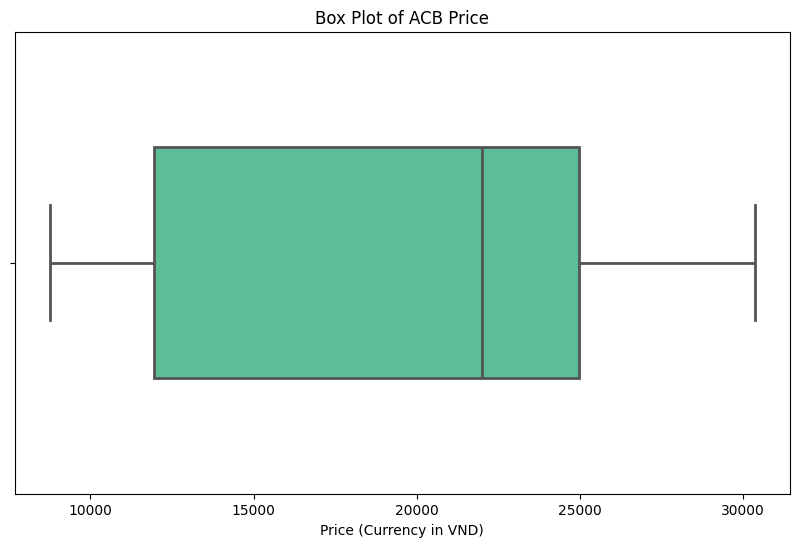
\includegraphics[width=1\textwidth]{bibliography/Figure/ACBboxplot.png}
    \caption{ACB stock price's boxplot}
    \label{fig:1}
    \end{minipage}
    \hfill
     \begin{minipage}{0.23\textwidth}
        \centering
        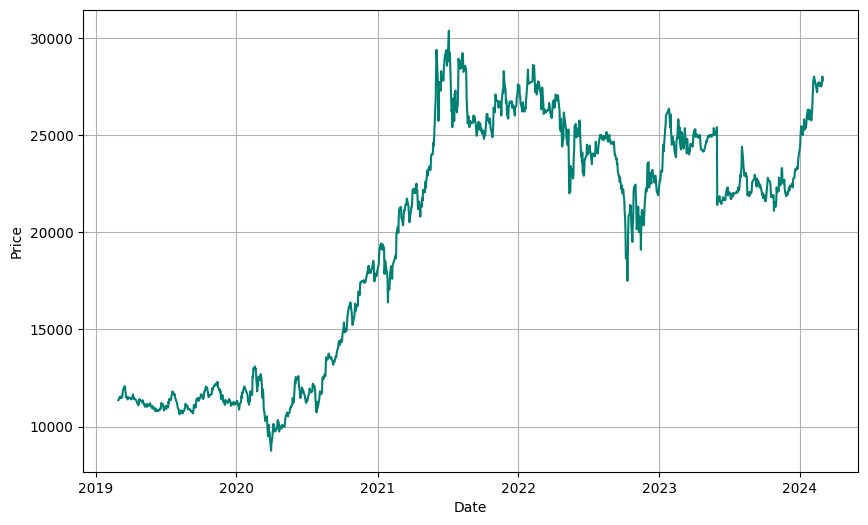
\includegraphics[width=\textwidth]{bibliography/Figure/ACBtime.png}
        \caption{ACB stock price's time}
        \label{fig:2}
    \end{minipage}
        \centering
    \begin{minipage}{0.23\textwidth}
    \centering
    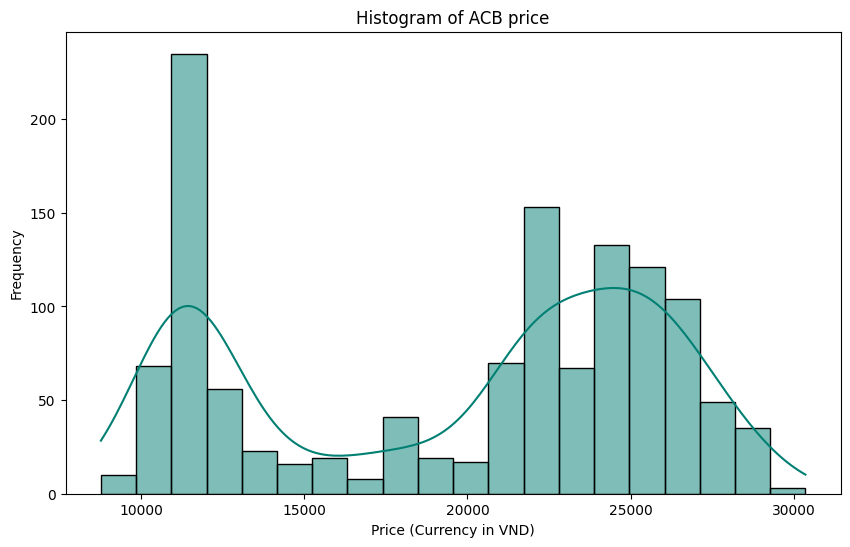
\includegraphics[width=1\textwidth]{bibliography/Figure/ACBhist.png}
    \caption{ACB stock price's histogram}
    \label{fig:3}
    \end{minipage}
\end{figure}
    ACB's price distribution appears left-skewed, as evidenced by the pronounced peak in the histogram at the lower end of the price range. Interestingly, ACB's box plot appears relatively compact, with the median closer to the higher end of the price range
\subsubsection{BID stock price visualization}
\begin{figure}[H]
    \centering
    \begin{minipage}{0.23\textwidth}
        \centering
        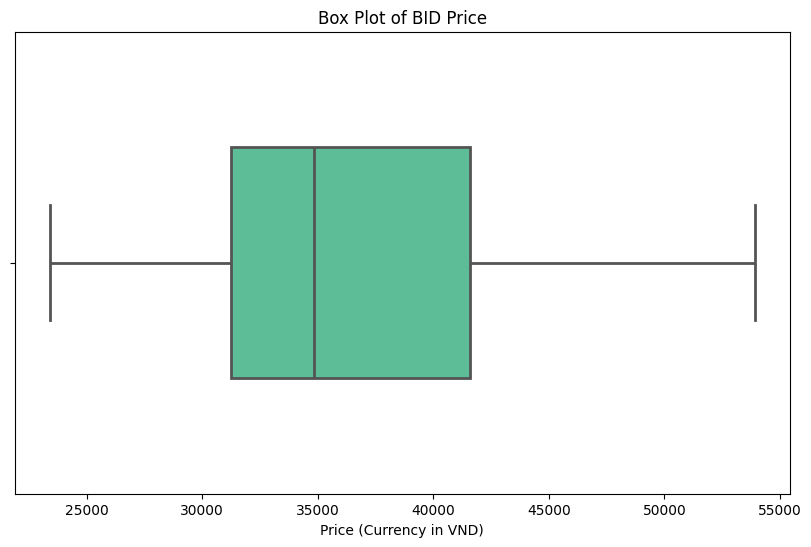
\includegraphics[width=1\textwidth]{bibliography/Figure/BIDboxplot.png}
        \caption{BID stock price's boxplot}
        \label{fig:1}
    \end{minipage}
    \hfill
    \begin{minipage}{0.23\textwidth}
        \centering
        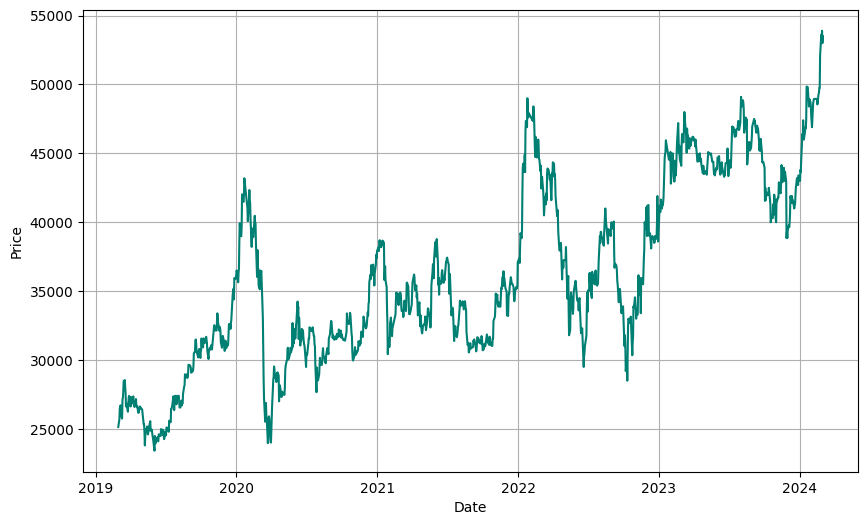
\includegraphics[width=\textwidth]{bibliography/Figure/BIDtime.png}
        \caption{BID stock price's time}
        \label{fig:2}
    \end{minipage}

    \end{figure}
    \begin{figure}[H]
    \centering
    \begin{minipage}{0.23\textwidth}
        \centering
        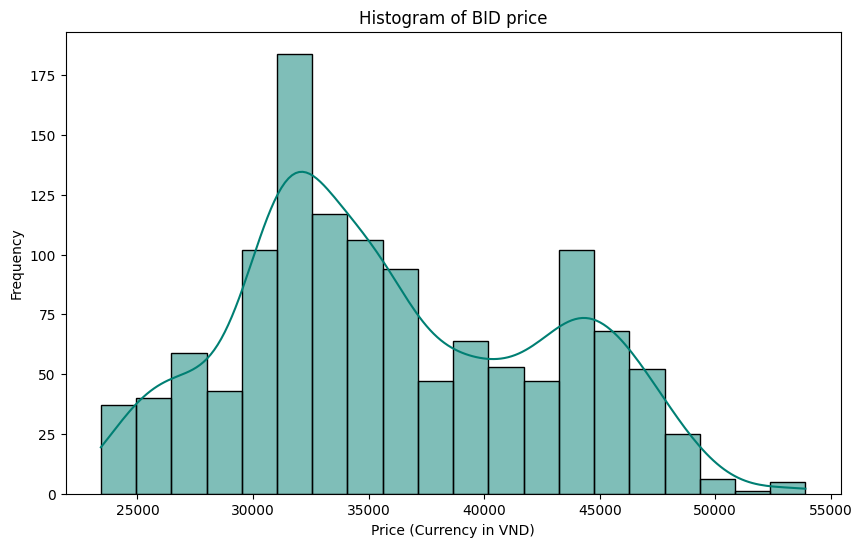
\includegraphics[width=1\textwidth]{bibliography/Figure/BIDhist.png}
        \caption{BID stock price's histogram}
        \label{fig:3}
    \end{minipage}
\end{figure}
The value of BID shares mainly fluctuates between 33,000 VND and 43,000 VND, and the highest current value that BID shares have reached is 54,000 VND. Additionally, the current trend regarding the value of BID shares is on the rise.
\subsubsection{VCB stock price visualization}
\begin{figure}[H]
    \centering
    \begin{minipage}{0.23\textwidth}
        \centering
        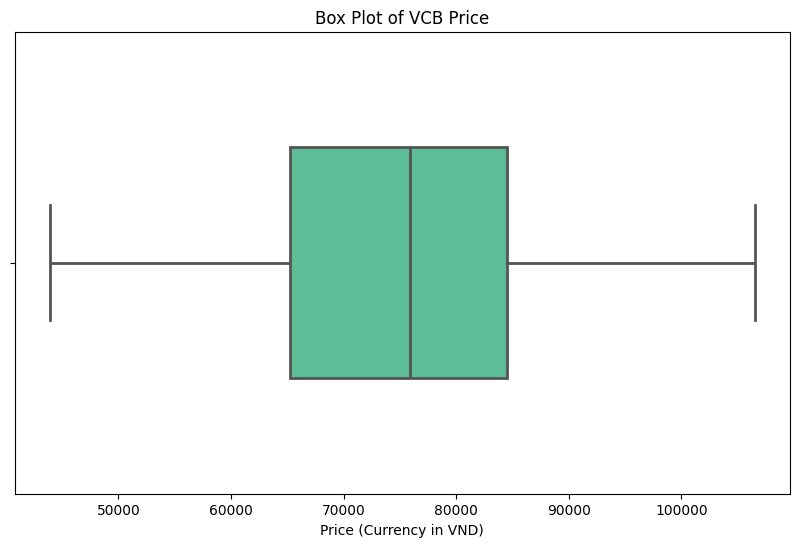
\includegraphics[width=1\textwidth]{bibliography/Figure/VCBboxplot.png}
        \caption{VCB stock price's boxplot}
        \label{fig:1}
    \end{minipage}
    \hfill
    \begin{minipage}{0.23\textwidth}
        \centering
        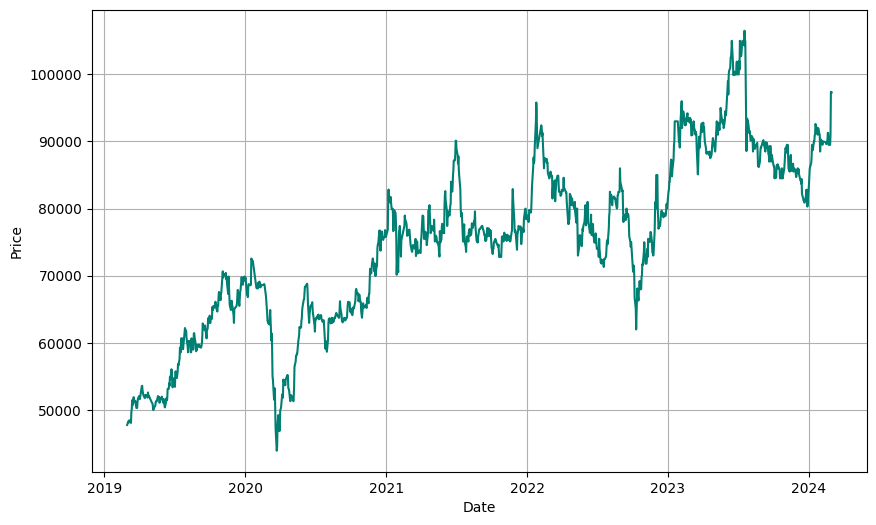
\includegraphics[width=1.1\textwidth]{bibliography/Figure/VCBtime.png}
        \caption{VCB stock price's time}
        \label{fig:2}
    \end{minipage}
    \begin{minipage}{0.23\textwidth}
        \centering
        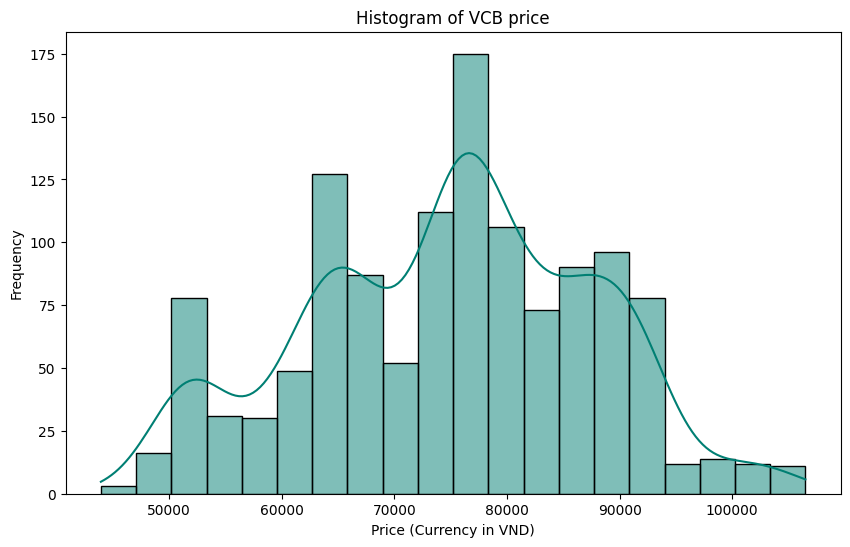
\includegraphics[width=\textwidth]{bibliography/Figure/VCBhist.png}
        \caption{VCB stock price's histogram}
        \label{fig:3}
    \end{minipage}
\end{figure}

% vcb boxplot
 Based on VCB's Boxplot, it can be seen that most of the data is concentrated in Q2 to Q3 with length 8654 approximately 75871 to 84525.
% vcb histogram
The highest concentration on the chart at the price of about 76,000 VND with a frequency of nearly 175 times may be a sign of investors' special interest in VCB stock price. Besides, the price also fluctuates frequently around 70,000
The data chart of price fluctuations over the years shows that stock prices tend to gradually increase, although prices also decrease to the lowest (43925) in early 2020 and the highest (106500) in mid-2023.
\section{Methodology}

\subsection{ARIMA}
Auto Regressive Integrated Moving Average (ARIMA) is a model that describes time series based on observed values, which can be used to forecast future values. Applying ARIMA models to any time series showing patterns with no random white noise and non-seasonality. The model was introduced by Box and Jenkins in 1970. To generate short-term forecasts, ARIMA models have shown efficient capabilities, outperforming complex structural models. The future value of a variable in the ARIMA model is a combination of linearity to the past values and errors, expressed as follows \cite{Gillian}:
\begin{equation*}
Y_t = \phi_0 + \phi_1 Y_{t-1} + \phi_2 Y_{t-2} + \ldots + \phi_p Y_{t-p} + \varepsilon_t - \theta_1 \varepsilon_{t-1} - \ldots - \theta_q \varepsilon_{t-q}
\end{equation*}

Where:
\begin{itemize}
    \item $Y_t$ is the actual value at time $t$.
    \item $\varepsilon_t$ is the random error at time $t$.
    \item $\phi_i$ and $\theta_j$ are the coefficients.
    \item $p$ and $q$ are integers, often referred to as autoregressive and moving average parameters, respectively.
\end{itemize}

% Linear
\subsection{Linear Regression}
Linear regression is a statistical technique used to model the relationship between a dependent variable, \textit{Y}, and one or more independent variables, \textit{X}. The goal is to find the best-fitting straight line (or hyperplane in higher dimensions) that describes the relationship between the variables. 
When there are multiple independent variables, the linear regression is called multivariable linear regression, with equation has the form \cite{busin}:
 \[Y=\beta_0+\beta_1X_1+\beta_2X_2+\cdots+\beta_kX_k+\varepsilon\]
 
Where:\\
	\indent\textbullet\ Y is the dependent variable.\\
	\indent\textbullet\ \(X_1, X_2, \ldots, X_k\) are the independent variables.\\
	\indent\textbullet\ \(\beta_0\) is the intercept term.\\
	\indent\textbullet\ \(\beta_1,..., \beta_k\) are the regression coefficients for the independent variables.\\
	\indent\textbullet\ \(\varepsilon\) is the error term.

\subsection{FAST FOURIER TRANSFORM}
The Fast Fourier Transform (commonly abbreviated as
FFT) is a fast algorithm for computing the discrete Fourier
transform (DFT) of a sequence \cite{Gillian} by using the factor N/2
log N where N is the number of points, therefore, the FFT is a
way to convert the time series from time domain to frequency
domain \cite{Musbah} with equation \cite{Roberts}: 
\[
X[k] = \sum_{n=0}^{N-1} x[n] \cdot e^{-i \frac{2\pi}{N} kn}
\]
\\
Where:
\begin{itemize}
    \item $X[k]$ is the Discrete Fourier Transform of the sequence.
    \item $ x[n]$ is the $n$-th element of the input sequence.
    \item $N$ is the total number of elements in the input sequence.
    \item \( k \): Index variable ranging from \( 0 \) to \( N-1 \), representing the frequency index in the output sequence \( X[k] \).
\end{itemize}

Discrete Fourier Transform (DFT) of an \( N \)-point sequence requires \( O(N^2) \) operations. When \( N \) increases, this approach becomes impractically slow. Instead, Fast Fourier Transforms (FFT) offer efficient algorithms for computing DFTs in \( O(N \log N) \) operations.

Dart library uses Radix2FFT - a member of the family of so called Fast Fourier transform (FFT) algorithms, this implementation for power of two FFTs that is much faster than the other implementations by using Cooley-Tukey \cite{dark}. It computes separately the DFTs of the even-indexed inputs (\( x_0, x_2, \ldots, x_{N-2} \)) and of the odd-indexed inputs (\( x_1, x_3, \ldots, x_{N-1} \)), and then combines those two results to produce the DFT of the whole sequence \cite{radix}:

\[
X[k] = \sum_{m=0}^{\frac{N}{2}-1} x(2m) e^{-\frac{2\pi i}{N} (2m)k} + \sum_{m=0}^{\frac{N}{2}-1} x(2m+1) e^{-\frac{2\pi i}{N} (2m+1)k}\]
\\Where : 
\begin{itemize}
    \item $X[k]$: Represents the \( k \)-th element of the Discrete Fourier Transform (DFT) output sequence.
    \item \( m \): Index variable ranging from \( 0 \) to \( \frac{N}{2}-1 \). It denotes the position within the input sequence \( x \).
    \item \( x(2m) \) and \( x(2m+1) \): Elements of the input sequence \( x \) at indices \( 2m \) (even-indexed) and \( 2m+1 \) (odd-indexed), respectively. These are the values of the input sequence at specific positions determined by \( m \).
    \item \( k \): Index variable representing the frequency component in the output sequence \( X[k] \) can be represented by the DFT output, typically from \( 0 \) to \( N-1 \).
    \item \( e^{-\frac{2\pi i}{N} (2m)k} \) and \( e^{-\frac{2\pi i}{N} (2m+1)k} \): Complex exponential factors corresponding to the DFT calculation. These factors encode the phase shifts applied to each input element \( x(2m) \) and \( x(2m+1) \) to compute their contributions to the DFT output \( X[k] \).
\end{itemize}

\subsection{XGBoost}
XGBoost is a highly efficient and scalable implementation of gradient boosting, a powerful machine learning technique. XGBoost operates by constructing a series of decision trees in an additive manner. Each tree is built sequentially, with each one correcting the errors of the previous trees. Key advantages of XGBoost include its ability to handle large datasets through parallelized computing, effective handling of missing data values, and regularization techniques to prevent overfitting\cite{Xgboost}.The model’s objective is to minimize the loss function. 

Explanation of the mathematics behind XGBoost:\\
\textbf{Ensemble Model:} XGBoost combines predictions from multiple decision trees $(f_k)$ to create a final prediction (F(x))\cite{Xgboost}:

\begin{equation*}
\hat{y}_i = \sum_{k=1}^n f_k(x_i), \quad f_k \in \mathcal{F},
\end{equation*}
Where:
\begin{itemize}
\item \(\mathcal{F}\) means the space of regression trees, 
\item \( f_k \) corresponds to a tree,
\item \( f_k(x_i) \) is the result of tree \( k \),
\item \( \hat{y}_i \) is the predicted value of the \( i \)th instance \( x_i \).
\end{itemize}

\begin{figure}[H]
    \centering
\begin{minipage}{0.4\textwidth}
        \centering
        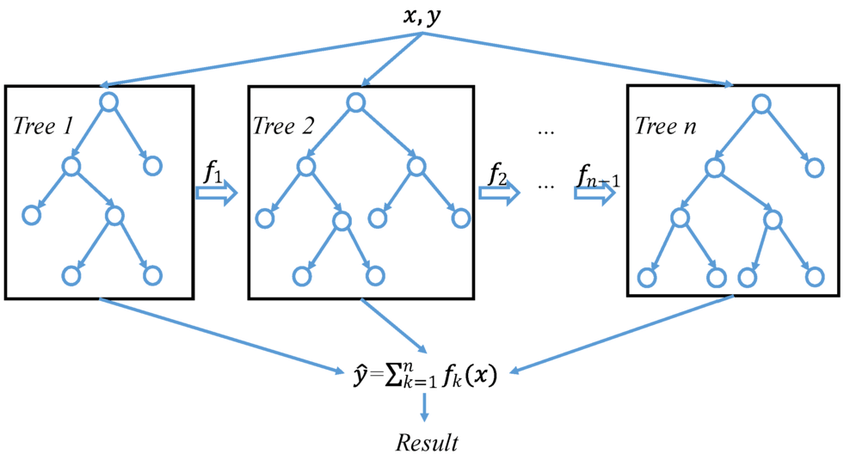
\includegraphics[width=\textwidth]{bibliography/Figure/xgboost.png}
        \caption{A general architecture of XGBoost}
        \label{fig:3}
\end{minipage}
\end{figure}

\textbf{Objective Function:}
It minimizes a loss function (L) that measures prediction error, with a regularization term ($\Omega$) to prevent overfitting:\cite{geekXGboost}

\begin{equation*}
\text{obj}(\theta) = L(\theta) + \Omega(\theta)
\end{equation*}

Where:
\begin{itemize}
    \item \( L(\theta) = \sum_{i=1}^n l(y_i, \hat{y}_i) \) is the loss function, \(\hat{y}_i\) is the prediction and \( y_i \) is the target
    \item \( \Omega(\theta) = \sum_{k=1}^K \Omega(f_k) \) penalizes the complexity of the model
\end{itemize}
\subsection{Recurrent neural network (RNN)}
A recurrent neural network (RNN) is a type of artificial neural network which uses sequential data or time series data\cite{IBM}.  A recurrent neural network (RNN) is an extension of a conventional feedforward neural network, which is able to handle a variable-length sequence input. The RNN handles the variable-length sequence by having a recurrent hidden state whose activation at each time is dependent on that of the previous time\cite{Chung}.
For each timestep \( t \), the activation \( a^{<t>} \) and the output \( y^{<t>} \) are expressed as follows:
\[
a^{<t>} = g_1\left( W_{aa} a^{<t-1>} + W_{ax} x^{<t>} + b_a \right)
\]
and
\[
y^{<t>} = g_2\left( W_{ya} a^{<t>} + b_y \right)
\]
where \( W_{ax}, W_{aa}, W_{ya}, b_a, b_y \) are coefficients that are shared temporally and \( g_1, g_2 \) are activation functions \cite{standford}.

\begin{figure}[H]
    \centering
\begin{minipage}{0.5\textwidth}
        \centering
        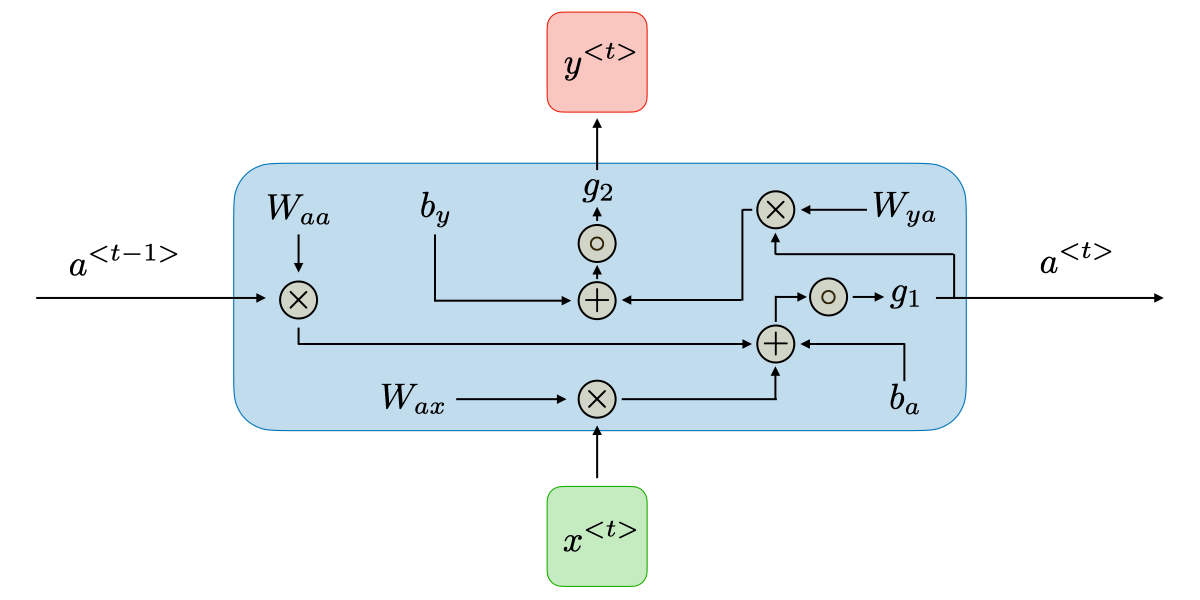
\includegraphics[width=\textwidth]{bibliography/Figure/RNNmodel.png}
        \caption{Architecture of a Traditional RNN}
        \label{fig:3}
\end{minipage}
\end{figure}

\subsection{Long short term memory (LSTM)}
The Long Short-Term Memory (LSTM) model is a recurrent neural network designed to handle sequential data like time series. Unlike standard RNNs, LSTMs employ memory cells and gating mechanisms to selectively retain and discard information over long sequences. This allows LSTMs to effectively capture long-range dependencies within the sequential data\cite{LSTM1}.

At the core of an LSTM are the memory cells regulated by gates - input gate (controls inflow), forget gate (controls clearing), and output gate (controls outflow). This gating architecture enables LSTMs to learn and leverage long-term patterns and relationships present in sequences. By addressing long-range temporal dependencies, LSTMs excel at sequence prediction tasks, making them well-suited for applications such as time series forecasting\cite{LSTM2}. 

\\\textbf{Forget gate}: Determine which information to discard from the cell state.
\begin{equation*}
f_t = \sigma(W_f \cdot [h_{t-1}, x_t] + b_f)
\end{equation*}

\\\textbf{Input Gate and Candidate Cell State}: Input gate($i_t$) regulates the new information stored in the cell state, while the candidate cell state ($\tilde{C}_t$) represents a filtered version of the input data.
\begin{equation*}
i_t = \sigma(W_i \cdot [h_{t-1}, x_t] + b_i)
\end{equation*}
\begin{equation*}
\tilde{C}_t = \tanh(W_c \cdot [h_{t-1}, x_t] + b_c) 
\end{equation*}

\\\textbf{Cell state update}: Drop the information about the old subject’s gender and add the new information,as determined in the previous steps.
\begin{equation*}
C_t = f_t \ast C_{t-1} + i_t \ast \tilde{C}_t
\end{equation*}

\textbf{Output gate}: Manages the parts of the cell state that are output to the next layer or used in the final prediction.
\begin{equation*}
o_t = \sigma(W_o \cdot [h_{t-1}, x_t] + b_o)
\end{equation*}
\begin{equation*}
h_t = o_t \ast \tanh(C_t)
\end{equation*}
\\Where:
\begin{itemize}
\item $i_t, f_t, o_t$ are the values of the gates at time $t$.
\item $W_i, W_f, W_o, W_C$ are weight matrices.
\item $b_i, b_f, b_o, b_c$ are bias vectors.
\item $h_{t-1}$ is the hidden state from the previous layer.
\item $x_t$ is the input at time $t$.
\item $C_t$ is the memory cell state at time $t$.
\item $h_t$ is the hidden state at time $t$.
\end{itemize}
\begin{figure}[H]
    \centering
    \begin{minipage}{0.5\textwidth}
        \centering
        \scalebox{0.7}[0.7]{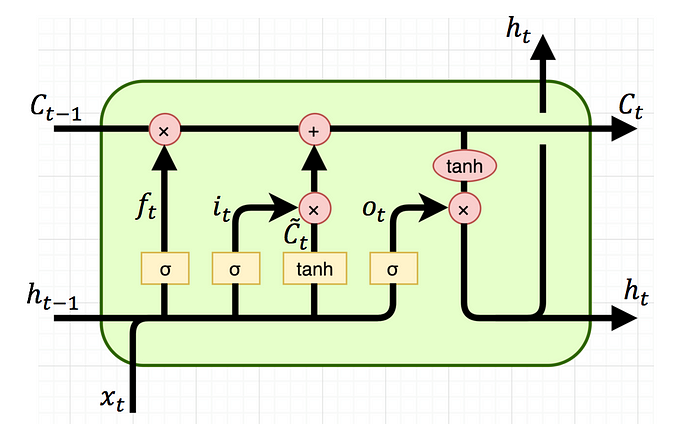
\includegraphics[width=\textwidth]{bibliography/Figure/LSTM.png}}
        \caption{Structure of the LSTM cell }
        \label{fig:3}
    \end{minipage}
\end{figure}
\subsection{GRU}


\begin{figure}[H]
    \centering
\begin{minipage}{0.4\textwidth}
        \centering
        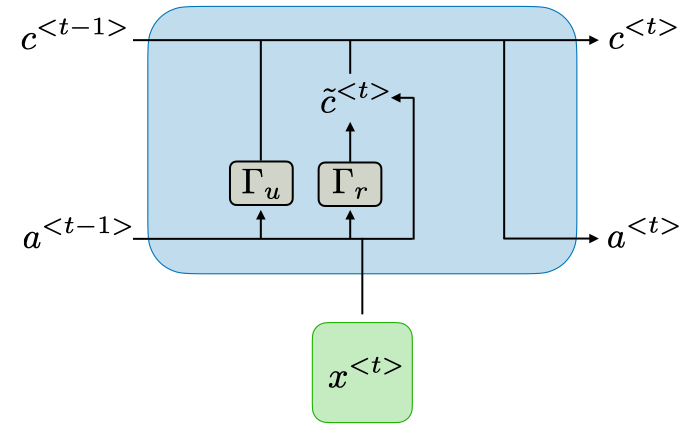
\includegraphics[width=\textwidth]{bibliography/Figure/gru-ltr.png}
        \caption{GRU architecture}
        \label{fig:3}
\end{minipage}
\end{figure}

\subsection{Fully Convolutional Network (FCN)}
Each layer output in a convnet is a three-dimensional array
of size $h \times w \times d$, where $h$ and $w$ are spatial dimensions, and
$d$ is the feature or channel dimension. The first layer is the
image, with pixel size $h \times w$, and $d$ channels. Locations in
higher layers correspond to the locations in the image they
are path-connected to, which are called their receptive fields.
Convnets are inherently translation invariant. Their basic components (convolution, pooling, and activation functions) operate on local input regions, and depend only on
relative spatial coordinates. Writing $x_{ij}$ for the data vector at
location $(i, j)$ in a particular layer, and $y_{ij}$ for the following
layer, these functions compute outputs $y_{ij}$ by:

\[
y_{ij} = f_{ks} \left( \{x_{si+\delta_i, sj+\delta_j}\}_{0 \le \delta_i, \delta_j < k} \right)
\]

where $k$ is called the kernel size, $s$ is the stride or subsampling factor, and $f_{ks}$ determines the layer type: a matrix
multiplication for convolution or average pooling, a spatial
max for max pooling, or an elementwise nonlinearity for an
activation function, and so on for other types of layers.
This functional form is maintained under composition,
with kernel size and stride obeying the transformation rule:

\[
f_{ks} \circ g_{k's'} = (f \circ g)_{k' + (k-1)s', ss'}
\]

While a general net computes a general nonlinear function,
a net with only layers of this form computes a nonlinear
filter, which we call a deep filter or fully convolutional network.
An FCN naturally operates on an input of any size, and
produces an output of corresponding (possibly resampled)
spatial dimensions.\cite{Ismail}

\begin{figure}[H]
    \centering
\begin{minipage}{0.5\textwidth}
        \centering
        \includegraphics[width=\textwidth]{bibliography/fcn.png}
        \caption{Fully Convolutional Neural Network architecture}
        \label{fig:3}
\end{minipage}
\end{figure}

\section{Result}
\subsection{Evaluation Methods}
\textbf{Mean Percentage Absolute Error} (MAPE): is the average percentage error in a set of predicted values\cite{Eval}.\\
\begin{equation*}
    MAPE=\frac{100\%}{n}  \sum_{i=1}^{n} |y_i-\hat{y_i} |  = 1 
\end{equation*}
\textbf{Root Mean Squared Error} (RMSE): is the square root of average value of squared error in a set of predicted values\cite{Eval}.
\begin{equation*}
    RMSE=\sqrt{\sum_{i=1}^{n} \frac{(\hat{y_i}-y_i )^2}{n} }
\end{equation*}
\textbf{Mean Absolute Error} (MAE): is the average absolute differences between the expected and actual values\cite{Eval}.
\begin{equation*}
    MAE= \frac{1}{n}\sum_{i=1}^{n}|y_i - \hat{g}_i|
\end{equation*}
Where:
\begin{itemize}
    \item \(n\) is the number of observations in the dataset
    \item \(y_i\)  is the true value
    \item \(\hat{y_i}\) is the predicted value
\end{itemize}
\subsection{ACB dataset}
\begin{table}[H]
    \centering
    \begin{tabular}{|c|c|c|c|c|}
         \hline
         \multicolumn{5}{|c|}{\textbf{Dataset's Evaluation}}\\
         \hline
         \centering Model & Proportion & RMSE & MAPE (\%) & MAE\\
\hline
\multirow{3}{*}{\centering ARIMA} & 7:3 & 3932.5798 & 13.7514 & 3308.4751 \\
     & 8:2 & 1542.0814 & 4.8217 & 1224.8404 \\
     & \textcolor{red}{9:1} & \textcolor{red}{1238.2448} & \textcolor{red}{3.8899} & \textcolor{red}{997.3804} \\
\hline
\multirow{3}{*}{\centering GRU}   & \textcolor{red}{7:3} & \textcolor{red}{380.5252} & \textcolor{red}{1.0507} & \textcolor{red}{244.9516} \\
     & 8:2 & 412.8149 & 1.0227 & 252.8959 \\
     & 9:1 & 545.3742 & 1.2304 & 332.2477 \\
\hline
\multirow{3}{*}{\centering FCN}   & \textcolor{red}{7:3} & \textcolor{red}{737.0995} & \textcolor{red}{2.6172} & \textcolor{red}{598.4848} \\
     & 8:2 & 1111.2461 & 3.6139 & 911.2206 \\
     & 9:1 & 827.6391 & 2.1990 & 588.7729 \\
\hline
\multirow{3}{*}{\centering RNN}   & 7:3 & 515.8307 & 1.6065 & 372.2723 \\
     & \textcolor{red}{8:2} & \textcolor{red}{497.3003} & \textcolor{red}{1.3553} & \textcolor{red}{334.5276} \\
     & 9:1 & 578.2733 & 1.4166 & 381.5157 \\
\hline
\multirow{3}{*}{\centering LSTM}  & 7:3 & 461.341 & 1.4958 & 341.2479 \\
     & \textcolor{red}{8:2} & \textcolor{red}{495.0181} & \textcolor{red}{1.3254} & \textcolor{red}{331.5678} \\
     & 9:1 & 580.2895 & 1.3335 & 359.7341 \\
\hline
\multirow{3}{*}{\centering FFT}   & 7:3 & 12366.0056 & 50.3046 & 11610.1708 \\
     & 8:2 & 4629.2061 & 18.8982 & 4397.2235 \\
     & \textcolor{red}{9:1} & \textcolor{red}{1909.2008} & \textcolor{red}{6.6089} & \textcolor{red}{1722.2856} \\
\hline
\multirow{3}{*}{\centering XGBOOST} & \textcolor{red}{7:3} & \textcolor{red}{402.127} & \textcolor{red}{1.2662} & \textcolor{red}{294.9247} \\
       & 8:2 & 448.5182 & 1.3043 & 322.6302 \\
       & 9:1 & 545.6544 & 1.4358 & 390.9168 \\
\hline
\multirow{3}{*}{\centering LR}    & 7:3 & 7607.3350 & 25.1283 & 7493.9168 \\
     & 8:2 & 3512.4495 & 11.5926 & 3100.1016 \\
     & \textcolor{red}{9:1} & \textcolor{red}{1797.1567} & \textcolor{red}{5.5612} & \textcolor{red}{1449.3335} \\
\hline
    \end{tabular}
    \caption{ACB Dataset's Evaluation}
    \label{vcbdataset}
\end{table}

For the ACB stock price prediction, GRU and XGBOOST model (both with a 7:3 proportion) appear to be the most accurate and reliable based on the the low
values in RMSE, MAPE, MAE. These models can potentially offer better insights and forecasting accuracy for investors dealing with ACB stocks in the Vietnamese market.
\begin{figure}[H]
    \centering
    \begin{minipage}{0.43\linewidth}
        \centering
        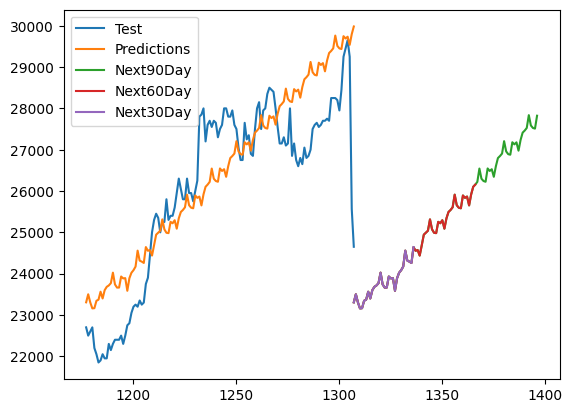
\includegraphics[width=\linewidth]{bibliography/diagram/ARIMA-ACB.png}
        \caption{ARIMA model’s result with 9:1 splitting proportion}
        \label{fig:ARIMA}
    \end{minipage}
    \hfill
    \begin{minipage}{0.43\linewidth}
        \centering
        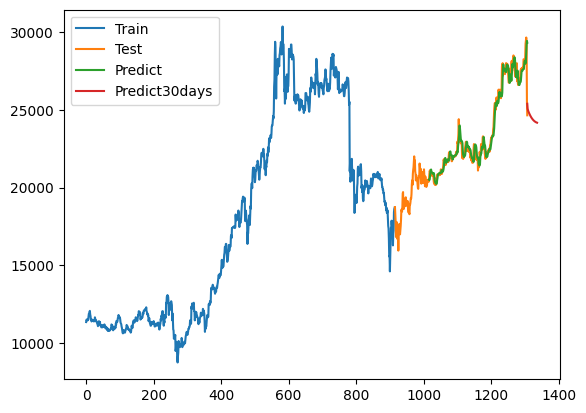
\includegraphics[width=\linewidth]{bibliography/diagram/GRU-ACB.png}
        \caption{GRU model’s result with 7:3 splitting proportion}
        \label{fig:GRU}
    \end{minipage}
\end{figure}
\begin{figure}[H]
    \centering
    \begin{minipage}{0.45\linewidth}
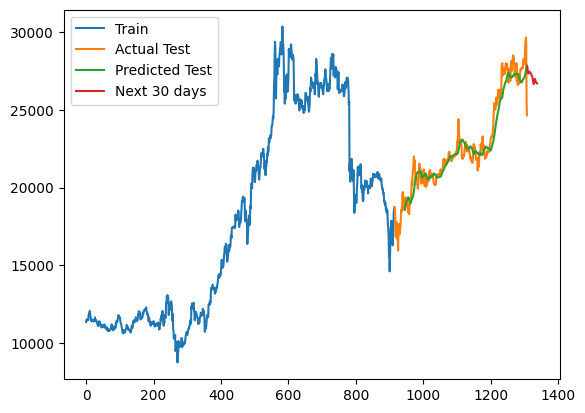
\includegraphics[width=\linewidth]{bibliography/diagram/FCN-ACB.png}
        \caption{FCN model’s result with 7:3 splitting proportion}
        \label{fig:FCN}
    \end{minipage}
    \hfill
    \begin{minipage}{0.45\linewidth}
        \centering
        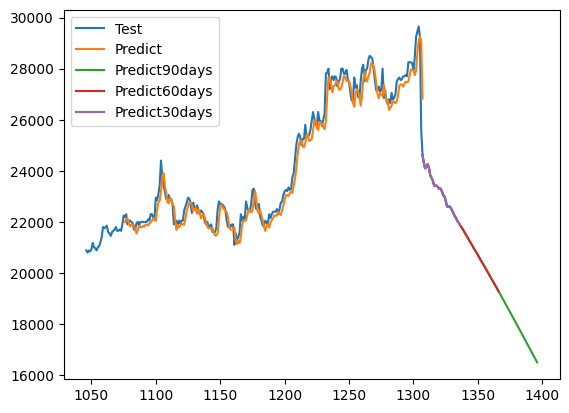
\includegraphics[width=\linewidth]{bibliography/diagram/RNN-ACB.png}
        \caption{RNN model’s result with 8:2 splitting proportion}
        \label{fig:RNN}
    \end{minipage}
\end{figure}
\begin{figure}[H]
    \centering
    \begin{minipage}{0.45\linewidth}
        \centering
        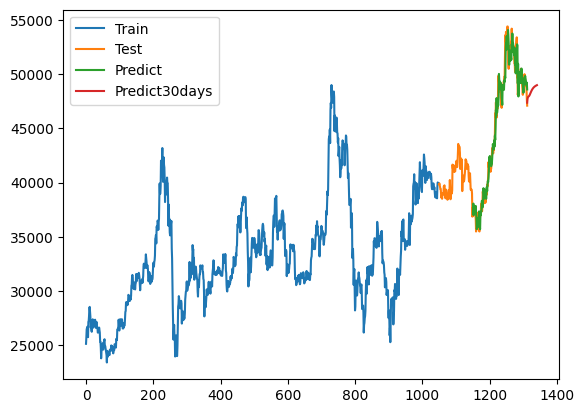
\includegraphics[width=\linewidth]{bibliography/diagram/LSTM-ACB.png}
        \caption{LSTM model’s result with 8:2 splitting proportion}
        \label{fig:LSTM}
    \end{minipage}
    \hfill
    \begin{minipage}{0.43\linewidth}
        \centering
        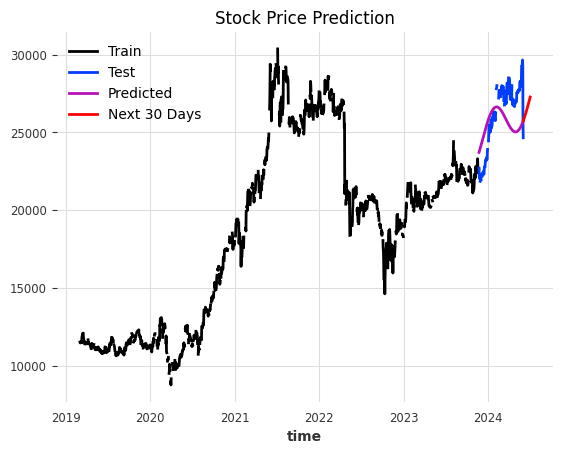
\includegraphics[width=\linewidth]{bibliography/diagram/FFT-ACB.png}
       \caption{FFT model’s result with 9:1 splitting proportion}
        \label{fig:FFT}
    \end{minipage}
\end{figure}
\begin{figure}[H]
    \centering
    \begin{minipage}{0.45\linewidth}
        \centering
    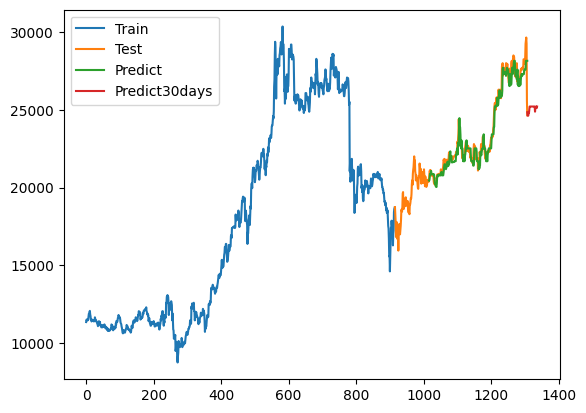
\includegraphics[width=\linewidth]{bibliography/diagram/XGBoost-ACB.png}
        \caption{XGBoost model’s result with 7:3 splitting proportion}
        \label{fig:XGBoost}
    \end{minipage}
    \hfill
    \begin{minipage}{0.45\linewidth}
        \centering
         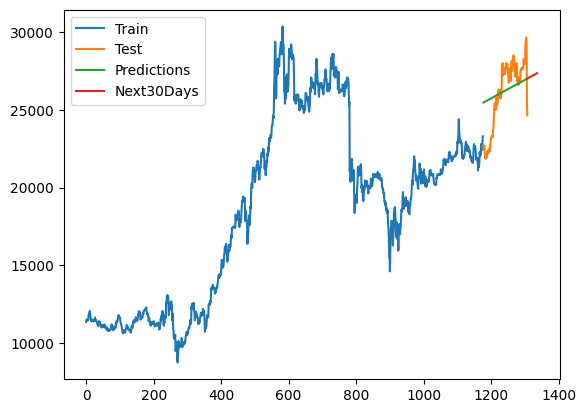
\includegraphics[width=\linewidth]{bibliography/diagram/LR-ACB.png}
        \caption{Linear Regression model’s result with 9:1 splitting proportion}
        \label{fig:LR}
    \end{minipage}
\end{figure}

\subsection{BID dataset} 

\begin{table}[H]
    \centering
    \begin{tabular}{|c|c|c|c|c|}
         \hline
         \multicolumn{5}{|c|}{\textbf{Dataset's Evaluation}}\\
         \hline
         \centering Model & Proportion & RMSE & MAPE (\%) & MAE\\
         \hline
         \multirow{3}{*}{ARIMA} 
         & 7:3 & 9563.7477 & 19.8847 & 8620.5906 \\ 
         & \textcolor{red}{8:2} & \textcolor{red}{6464.7779} & \textcolor{red}{10.0109} & \textcolor{red}{4764.1887} \\ 
         & 9:1 & 6158.2991 & 10.6520 & 5292.1888 \\
         \hline
         \multirow{3}{*}{GRU} 
         & \textcolor{red}{7:3} & \textcolor{red}{749.0815} & \textcolor{red}{1.2404} & \textcolor{red}{525.8805} \\ 
         & 8:2 & 782.4308 & 1.2474 & 552.8802 \\
         & 9:1 & 964.3091 & 1.3533 & 677.6551 \\
         \hline
         \multirow{3}{*}{FCN} 
         & 7:3 & 2259.3188 & 4.6895 & 1954.8440 \\ 
         & \textcolor{red}{8:2} & \textcolor{red}{1192.5075} & \textcolor{red}{1.9916} & \textcolor{red}{895.5052} \\ 
         & 9:1 & 1356.9802 & 2.0289 & 1015.2221 \\
         \hline
         \multirow{3}{*}{RNN} 
         & \textcolor{red}{7:3} & \textcolor{red}{1001.5601} & \textcolor{red}{1.8226} & \textcolor{red}{771.9509} \\ 
         & 8:2 & 1103.2342 & 2.0474 & 891.3108 \\ 
         & 9:1 & 1074.0008 & 1.6376 & 805.7158 \\
         \hline
         \multirow{3}{*}{LSTM} 
         & \textcolor{red}{7:3} & \textcolor{red}{820.0516} & \textcolor{red}{1.3974} & \textcolor{red}{593.1434} \\ 
         & 8:2 & 847.0286 & 1.3657 & 606.8658 \\ 
         & 9:1 & 1024.1498 & 1.4659 & 733.4891 \\
         \hline
         \multirow{3}{*}{FFT} 
         & \textcolor{red}{7:3} & \textcolor{red}{5736.0835} & \textcolor{red}{11.4603} & \textcolor{red}{4838.2472} \\
         & 8:2 & 5971.8017 & 11.4028 & 5100.2349 \\ 
         & 9:1 & 7792.9476 & 11.9885 & 6037.3514 \\
         \hline
         \multirow{3}{*}{XGBOOST} 
         & \textcolor{red}{7:3} & \textcolor{red}{3225.2175} & \textcolor{red}{4.2320} & \textcolor{red}{2005.3957} \\ 
         & 8:2 & 4007.5167 & 5.4957 & 2702.9580 \\ 
         & 9:1 & 6153.4990 & 10.9518 & 5571.4794 \\
         \hline
         \multirow{3}{*}{LR} 
         & \textcolor{red}{7:3} & \textcolor{red}{5967.7684} & \textcolor{red}{11.6453} & \textcolor{red}{1845.6229} \\
         & 8:2 & 6678.0104 & 12.9205 & 5097.8035 \\ 
         & 9:1 & 8699.7701 & 19.1198 & 7686.7608 \\
         \hline
    \end{tabular}
    \caption{BID Dataset's Evaluation}
    \label{vcbdataset}
\end{table}
Based on the evaluation table, the GRU model with an 7:3 training/testing ratio provides the best prediction results for BID stock prices, with the lowest RMSE (749.0815), MAPE (1.2404\%), and MAE (525.8805). LSTM is also a strong choice with similar performance at the same ratio. Overall, GRU stands out as the top choice for predicting BID stock prices

\begin{figure}[H]
    \centering
    \begin{minipage}{0.45\linewidth}
        \centering
        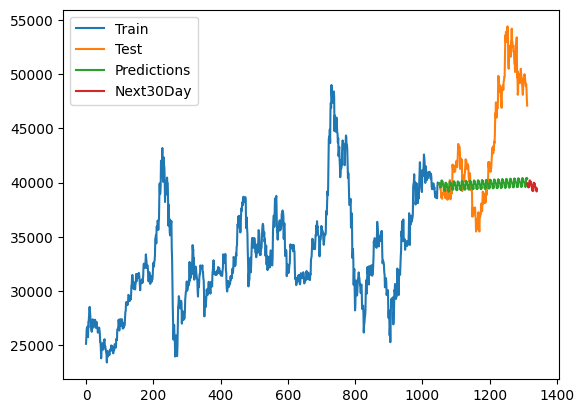
\includegraphics[width=\linewidth]{bibliography/diagram/ARIMA-BID.png}
        \caption{ARIMA model’s result with 8:2 splitting proportion}
        \label{fig:ARIMA-BID}
    \end{minipage}
    \hfill
    \begin{minipage}{0.45\linewidth}
        \centering
        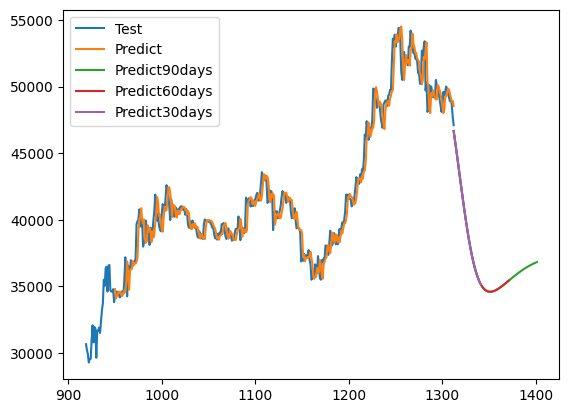
\includegraphics[width=\linewidth]{bibliography/diagram/GRU-BID.png}
        \caption{GRU model’s result with 7:3 splitting proportion}
        \label{fig:GRU-BID}
    \end{minipage}
\end{figure}

\begin{figure}[H]
    \centering
    \begin{minipage}{0.45\linewidth}
        \centering
        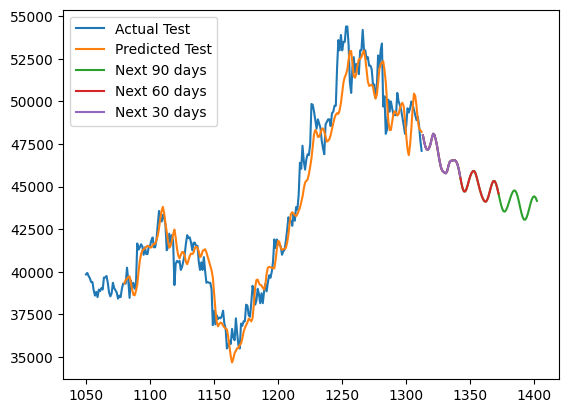
\includegraphics[width=\linewidth]{bibliography/diagram/FCN-BID.png}
        \caption{FCN model’s result with 8:3 splitting proportion}
        \label{fig:FCN-BID}
    \end{minipage}
    \hfill
    \begin{minipage}{0.45\linewidth}
        \centering
        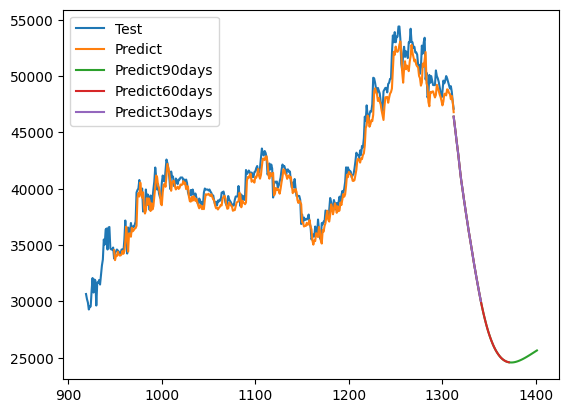
\includegraphics[width=\linewidth]{bibliography/diagram/RNN-BID.png}
        \caption{RNN model’s result with 7:3 splitting proportion}
        \label{fig:RNN-BID}
    \end{minipage}
\end{figure}

\begin{figure}[H]
    \centering
    \begin{minipage}{0.45\linewidth}
        \centering
        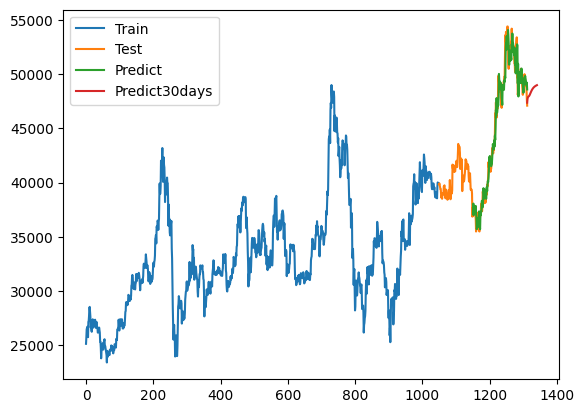
\includegraphics[width=\linewidth]{bibliography/diagram/LSTM-BID.png}
        \caption{LSTM model’s result with 7:3 splitting proportion}
        \label{fig:LSTM-BID}
    \end{minipage}
    \hfill
    \begin{minipage}{0.45\linewidth}
        \centering
        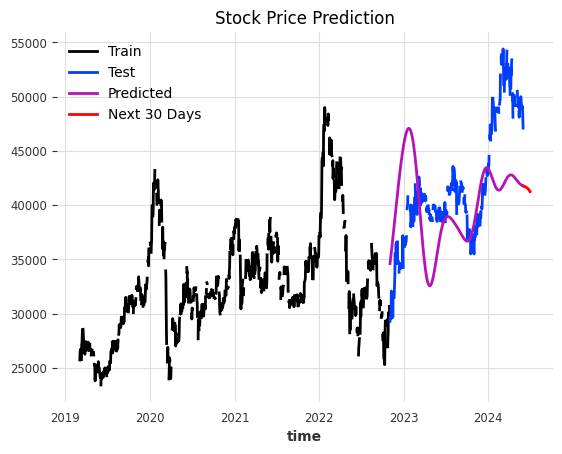
\includegraphics[width=\linewidth]{bibliography/diagram/FFT-BID.png}
        \caption{FFT model’s result with 7:3 splitting proportion}
        \label{fig:FFT-BID}
    \end{minipage}
\end{figure}

\begin{figure}[H]
    \centering
    \begin{minipage}{0.45\linewidth}
        \centering
        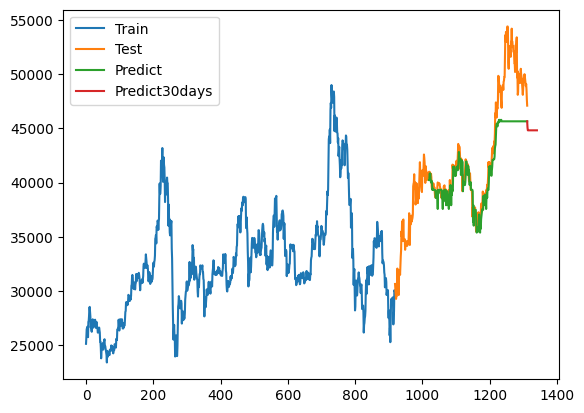
\includegraphics[width=\linewidth]{bibliography/diagram/XGBoost-BID.png}
        \caption{XGBoost model’s result with 7:3 splitting proportion}
        \label{fig:XGBoost-BID}
    \end{minipage}
    \hfill
    \begin{minipage}{0.45\linewidth}
        \centering
        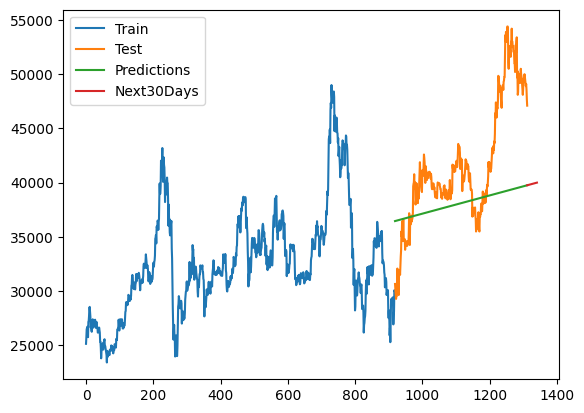
\includegraphics[width=\linewidth]{bibliography/diagram/LR-BID.png}
        \caption{Linear Regression model’s result with 7:3 splitting proportion}
        \label{fig:LR-BID}
    \end{minipage}
\end{figure}

\subsection{VCB dataset} 
\begin{table}[H]
    \centering
    \begin{tabular}{|c|c|c|c|c|}
         \hline
         \multicolumn{5}{|c|}{\textbf{Dataset's Evaluation}}\\
         \hline
         \centering Model & Proportion & RMSE & MAPE (\%) & MAE\\
         \hline
        \multirow{3}{*}{ARIMA} 
        & 7:3 & 39861.8637 & 41.9820 & 36312.4125 \\
        & 8:2 & 16889.0992 & 15.3808 & 13728.8500 \\
        & \textcolor{red}{9:1} & \textcolor{red}{1238.2448} & \textcolor{red}{3.8899} & \textcolor{red}{997.3810} \\
        \hline
        \multirow{3}{*}{GRU} 
        & 7:3 & 1164.3590 & {1.0174} & 857.2915 \\
        & \textcolor{red}{8:2} & \textcolor{red}{1138.5327} & \textcolor{red}{0.9145} & \textcolor{red}{815.9355} \\
        & 9:1 & 1398.7836 & 1.0759 & 984.8921 \\
        \hline
        \multirow{3}{*}{FCN} 
        & 7:3 & 3824.7088 & 3.6075 & 3154.3828 \\
        & 8:2 & 4811.8376 & 4.9807 & 4469.9363 \\
        & \textcolor{red}{9:1} & \textcolor{red}{2732.1560} & \textcolor{red}{2.3252} & \textcolor{red}{2142.9079} \\
        \hline
        \multirow{3}{*}{RNN} 
        & 7:3 & 1619.5683 & 1.5273 & 1282.0946 \\
        & 8:2 & 1743.8729 & 1.5051 & 1326.5244 \\
        & \textcolor{red}{9:1} & \textcolor{red}{1254.2616} & \textcolor{red}{0.9490} & \textcolor{red}{855.2889} \\
        \hline
        \multirow{3}{*}{LSTM} 
        & 7:3 & 1697.3167 & 1.5419 & 1320.1187 \\
        & \textcolor{red}{8:2} & \textcolor{red}{1151.5582} & \textcolor{red}{0.9525} & \textcolor{red}{847.6950} \\
        & 9:1 & 1405.7421 & 1.0667 & 977.9067 \\
        \hline
        \multirow{3}{*}{FFT} 
        & \textcolor{red}{7:3} & \textcolor{red}{7654.6091} & \textcolor{red}{8.0921} & \textcolor{red}{6359.1013} \\
    
        & 8:2 & 10661.2453 & 10.5581 & 9399.3536 \\
       
        & 9:1 & 9141.6520 & 8.1522 & 7465.4590 \\
         \hline
        \multirow{3}{*}{XGBOOST} 
        & 7:3 & 3716.7589 & 3.0326 & 2705.8227 \\
        & 8:2 & 4671.1649 & 4.0999 & 3751.2325 \\
        & \textcolor{red}{9:1} & \textcolor{red}{3350.2323} & \textcolor{red}{2.9121} & \textcolor{red}{2708.4345} \\
        \hline
        \multirow{3}{*}{LR} 
        & 7:3 & 6987.9849 & 7.1427 & 5818.5129 \\
        & 8:2 & 9168.4296 & 10.5427 & 8439.4780 \\
        & \textcolor{red}{9:1} & \textcolor{red}{6673.7497} & \textcolor{red}{6.9101} & \textcolor{red}{5853.9128} \\
        \hline
    \end{tabular}
    \caption{VCB Dataset's Evaluation}
    \label{vcbdataset}
\end{table}
Based on the error metrics table for predicting VCB stock prices, GRU emerges as the most accurate model with an 8:2 data split. RNN and LSTM also achieve high accuracy, with RNN performing best in the 9:1 split and LSTM performing best in the 8:2 split. Although ARIMA shows the best performance in the 9:1 split, it still lags behind neural network models like GRU, RNN, and LSTM. FFT and LR, despite some improvement in certain cases, exhibit high and unstable errors, indicating they are less suitable for this dataset.

\begin{figure}[H]
    \centering
    \begin{minipage}{0.45\linewidth}
        \centering
        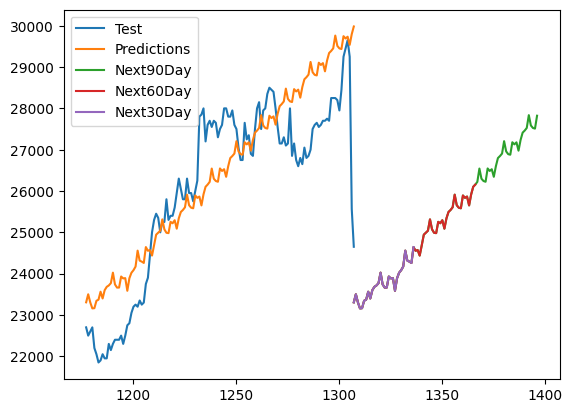
\includegraphics[width=\linewidth]{bibliography/diagram/ARIMA-VCB.png}
        \caption{ARIMA model’s result with 9:1 splitting proportion}
        \label{fig:ARIMA-VCB}
    \end{minipage}
    \hfill
    \begin{minipage}{0.45\linewidth}
        \centering
        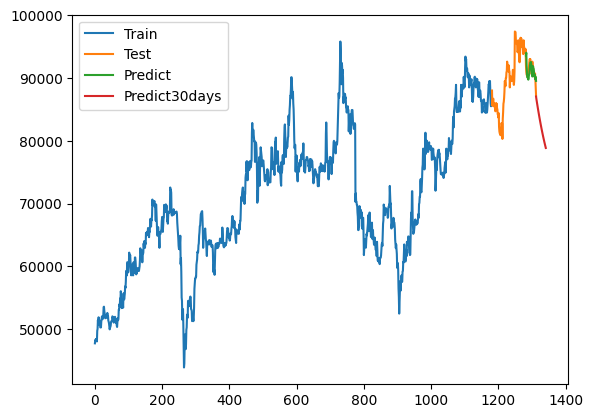
\includegraphics[width=\linewidth]{bibliography/diagram/GRU-VCB.png}
        \caption{GRU model’s result with 9:1 splitting proportion}
        \label{fig:GRU-VCB}
    \end{minipage}
\end{figure}

\begin{figure}[H]
    \centering
    \begin{minipage}{0.45\linewidth}
        \centering
        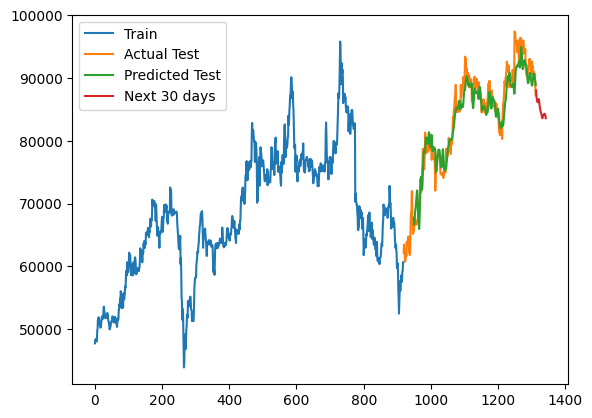
\includegraphics[width=\linewidth]{bibliography/diagram/FCN-VCB.png}
        \caption{FCN model’s result with 7:3 splitting proportion}
        \label{fig:FCN-VCB}
    \end{minipage}
    \hfill
    \begin{minipage}{0.45\linewidth}
        \centering
        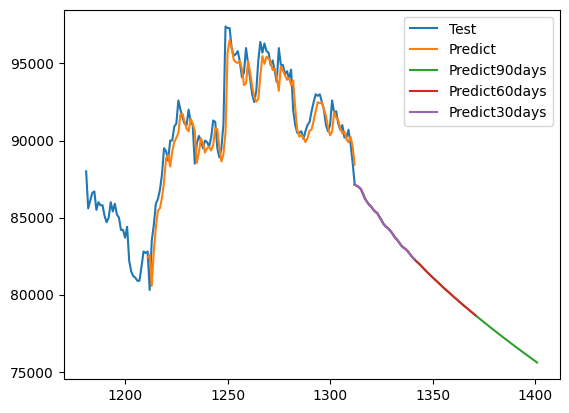
\includegraphics[width=\linewidth]{bibliography/diagram/RNN-VCB.png}
        \caption{RNN model’s result with 9:1 splitting proportion}
        \label{fig:RNN-VCB}
    \end{minipage}
\end{figure}

\begin{figure}[H]
    \centering
    \begin{minipage}{0.45\linewidth}
        \centering
        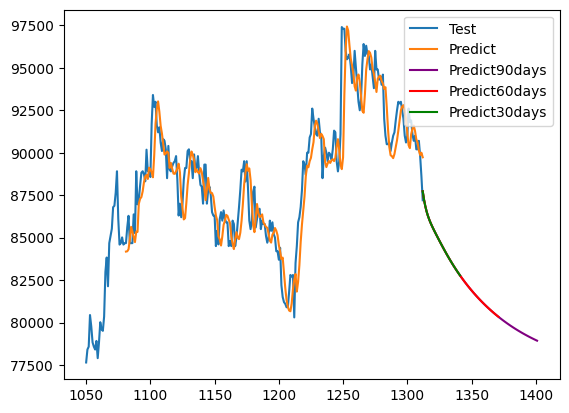
\includegraphics[width=\linewidth]{bibliography/diagram/LSTM-VCB.png}
        \caption{LSTM model’s result with 8:2 splitting proportion}
        \label{fig:LSTM-VCB}
    \end{minipage}
    \hfill
    \begin{minipage}{0.45\linewidth}
        \centering
        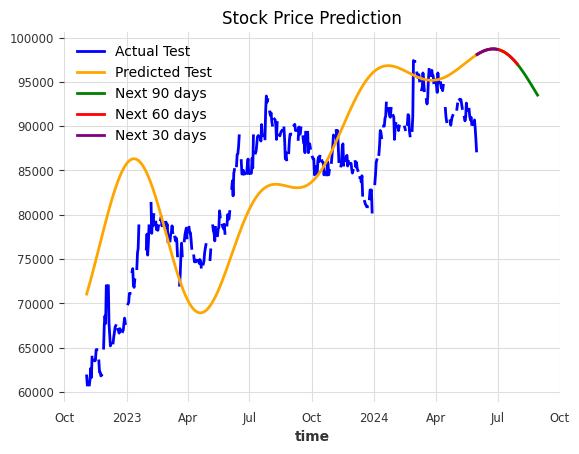
\includegraphics[width=\linewidth]{bibliography/diagram/FFT-VCB.png}
        \caption{FFT model’s result with 7:3 splitting proportion}
        \label{fig:FFT-VCB}
    \end{minipage}
\end{figure}

\begin{figure}[H]
    \centering
    \begin{minipage}{0.45\linewidth}
        \centering
        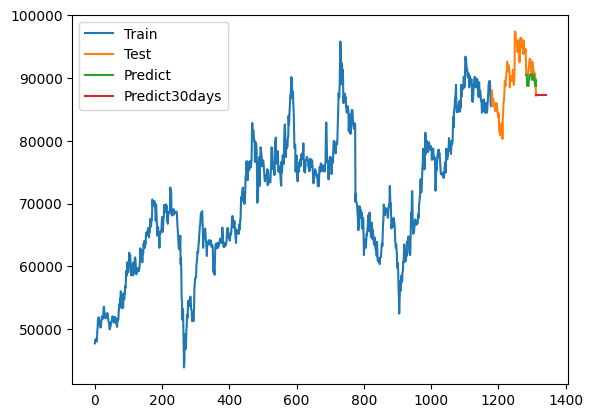
\includegraphics[width=\linewidth]{bibliography/diagram/XGBoost-VCB.png}
        \caption{XGBoost model’s result with 9:1 splitting proportion}
        \label{fig:XGBoost-VCB}
    \end{minipage}
    \hfill
    \begin{minipage}{0.45\linewidth}
        \centering
        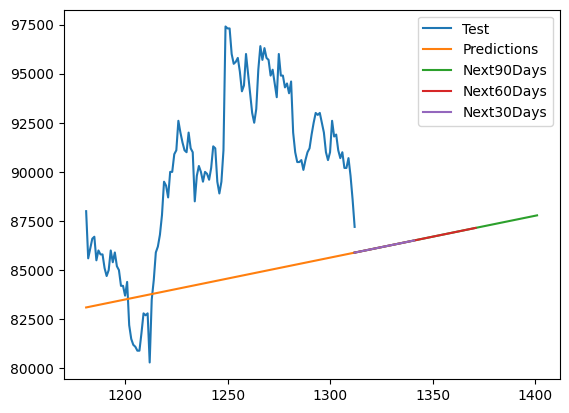
\includegraphics[width=\linewidth]{bibliography/diagram/LR-VCB.png}
        \caption{LR model’s result with 9:1 splitting proportion}
        \label{fig:LR-VCB}
    \end{minipage}
\end{figure}
% UNCOMMENT these lines below (and remove the 2 commands above) if you want to embed the bibliografy.



\section{Conclusion}
This research investigates the application of various machine learning and statistical models for stock price prediction, specifically focusing on ARIMA, GRU, FCN, RNN, LSTM, FFT, XGBoost, and Linear Regression. The study evaluates the performance of these models across three datasets (ACB, BID, and VCB) with three train-test ratios (7:3, 8:2, and 9:1). The models are assessed using common evaluation metrics: RMSE (Root Mean Squared Error), MAPE (Mean Absolute Percentage Error), and MAE (Mean Absolute Error).

GRU, FCN, RNN, LSTM, and XGBoost have lower evaluation metrics compared to the other models, indicating more accurate and efficient predictions. Specifically, XGBoost delivers the best results for the ACB dataset, outperforming other models in predicting ACB stock prices. XGBoost, with its ability to handle complex relationships and high performance on large datasets, shows strong potential for stock trend prediction.

Meanwhile, GRU demonstrates superior performance in predicting stock prices for BID and VCB. With its capability to capture sequential dependencies and process complex sequential data, GRU stands out in predicting the fluctuation patterns in the stock markets of BID and VCB. RNN also shows impressive performance, particularly in handling sequential data, helping to capture effective time-series patterns.
\section{ORIENTATION}
In the future, this research could expand in several promising directions. Integrating more advanced deep learning architectures than those currently studied could bring new insights. Models such as BERT (Bidirectional Encoder Representations from Transformers) or T5 (Text-To-Text Transfer Transformer), based on Transformer technology, have demonstrated outstanding capabilities in natural language processing and could be beneficial for predicting stock prices by capturing complex relationships within contexts.

Furthermore, incorporating richer external data sources beyond stock price history alone, such as broader economic indicators, sentiment analysis from news, or alternative data streams, could enrich the models' inputs and enhance their predictive abilities across diverse market conditions.

\section{Acknowledgment}
\addcontentsline{toc}{section}{Acknowledgment}
First and foremost, we would like to express our heartfelt gratitude to Associate Professors. \textbf{Prof. Dr. Nguyen Dinh Thuan} have given profound knowledge, critical insights, and attention to detail throughout the research
 process. In addition, \textbf{Mr. Nguyen Minh Nhut} directly provided dedicated instruction, and offered many valuable suggestions that helped our team in shaping the direction and quality of this report.

This report would not have been possible without the
 support and contributions of our mentors. Thank you all for your invaluable assistance and
 encouragement. We hope to that we will continue to receive support and encouragement from Associate Professors in the future.
\begin{thebibliography}{00}
\bibitem{cakra2015stock}
Cakra, Y. E., \& Trisedya, B. D. (2015, October). Stock price prediction using linear regression based on sentiment analysis. In 2015 international conference on advanced computer science and information systems (ICACSIS) (pp. 147-154). IEEE.
\bibitem{uras2020forecasting}
Uras, N., Marchesi, L., Marchesi, M., \& Tonelli, R. (2020). Forecasting Bitcoin closing price series using linear regression and neural networks models. PeerJ Computer Science, 6, e279.
\bibitem{dadhich2021predictive}
Dadhich, M., Pahwa, M. S., Jain, V., \& Doshi, R. (2021). Predictive models for stock market index using stochastic time series ARIMA modeling in emerging economy. In Advances in Mechanical Engineering: Select Proceedings of CAMSE 2020 (pp. 281-290). Springer Singapore.
\bibitem{garlapati2021stock}
Garlapati, A., Krishna, D. R., Garlapati, K., Rahul, U., \& Narayanan, G. (2021, April). Stock price prediction using Facebook Prophet and Arima models. In 2021 6th International Conference for Convergence in Technology (I2CT) (pp. 1-7). IEEE.
\bibitem{ZhuRNN}
Zhu, Y. (2020, October). Stock price prediction using the RNN model. In Journal of Physics: Conference Series (Vol. 1650, No. 3, p. 032103). IOP Publishing.
\bibitem{DingGRU}
Ding, X., Zhang, Y., Liu, T., \& Duan, J. (2015, June). Deep learning for event-driven stock prediction. In Twenty-fourth international joint conference on artificial intelligence.
\bibitem{ShejulGRU}
Shejul, A. A., Chaudhari, A., Dixit, B. A., \& Lavanya, B. M. (2023). Stock Price Prediction Using GRU, SimpleRNN and LSTM. In Intelligent Systems and Applications: Select Proceedings of ICISA 2022 (pp. 529-535). Singapore: Springer Nature Singapore.
\bibitem{fjellstrom2022lstm}
Fjellström, C. (2022, December). Long short-term memory neural network for financial time series. In 2022 IEEE International Conference on Big Data (Big Data) (pp. 3496-3504). IEEE.
\bibitem{ChenFFT}
Chen, M. Y., \& Chen, B. T. (2014). Online fuzzy time series analysis based on entropy discretization and a Fast Fourier Transform. Applied Soft Computing, 14, 156-166.

\bibitem{chen2016xgboost}
Chen, T., & Guestrin, C. (2016, August). Xgboost: A scalable tree boosting system. In Proceedings of the 22nd ACM SIGKDD International Conference on Knowledge Discovery and Data Mining (pp. 785-794).
\bibitem{nabiee2023stock}
Nabiee, S., \& Bagherzadeh, N. (2023). Stock Trend Prediction: A Semantic Segmentation Approach. arXiv preprint arXiv:2303.09323.


% IV
\bibitem{Gillian}
Smith, G. (2019). The fast fourier transform and its applications. Edingburgh: University of Edingburg.




\bibitem{Musbah}
Musbah, H., El-Hawary, M., \& Aly, H. (2019, October). Identifying seasonality in time series by applying fast fourier transform. In 2019 IEEE Electrical Power and Energy Conference (EPEC) (pp. 1-4). IEEE.

\bibitem{Roberts}
S.J. Roberts. "Lecture 7 - The Discrete Fourier Transform".
\bibitem{dark}
fftea. (n.d.). Dart packages. Retrieved June 21, 2024, from \url{https://pub.dev/packages/fftea}

\bibitem{radix} 
University of Connecticut. (2019). Radix-2 fast Fourier transform. Retrieved June 21, 2024, from \url{https://www.phys.uconn.edu/~rozman/Courses/m3511_19s/downloads/radix2fft.pdf}
\bibitem{busin}
Evans, J. R. (2017). Business analytics: Methods, models, and decisions. Pearson.

\bibitem{Xgboost}
Chen, T., \& Guestrin, C. (2016, August). Xgboost: A scalable tree boosting system. In Proceedings of the 22nd ACM SIGKDD International Conference on Knowledge Discovery and Data Mining (pp. 785-794).

\bibitem{geekXGboost}
P. Pawangfg. (n.d.). XGBoost. GeeksforGeeks. Retrieved February 6, 2023, from https://www.geeksforgeeks.org/xgboost/.

%GRU
\bibitem{Yamak}
Shiri, F. M., Perumal, T., Mustapha, N., \& Mohamed, R. (2023). A comprehensive overview and comparative analysis on deep learning models: CNN, RNN, LSTM, GRU. arXiv preprint arXiv:2305.17473.
%FCN
\bibitem{Ismail}
Long, J., Shelhamer, E., \& Darrell, T. (2015). Fully convolutional networks for semantic segmentation. In Proceedings of the IEEE conference on computer vision and pattern recognition (pp. 3431-3440).

\bibitem{Eval}
González-Sopeña, J. M., Pakrashi, V., \& Ghosh, B. (2021). An overview of performance evaluation metrics for short-term statistical wind power forecasting. Renewable and Sustainable Energy Reviews, 138, 110515.
% RNN
\bibitem{IBM}
IBM Technology company, “What are recurrent neural networks?”, Available at: \url{https://www.ibm.com/topics/recurrent-neural-networks}
\bibitem{Chung}
Chung, J., Gulcehre, C., Cho, K., \& Bengio, Y. (2014). Empirical evaluation of gated recurrent neural networks on sequence modeling. arXiv preprint arXiv:1412.3555.
\bibitem{standford}
A. Amidi and S. Amidi, "Recurrent Neural Networks Cheatsheet," Stanford University, [Online].

\bibitem{LSTM1}
Olah, C. (2015, August 27). Understanding LSTM Networks. Retrieved June 20, 2024, from https://colah.github.io/posts/2015-08-Understanding-LSTMs/.

\bibitem{LSTM2}
Van Houdt, G., Mosquera, C., & Nápoles, G. (2020). A Review on the Long Short-Term Memory Model. Artificial Intelligence Review, 54(1), 1-27. https://doi.org/10.1007/s10462-020-09838-1



\end{thebibliography}




%%%%%%%%%%%%%%%


\EOD

\end{document}
